\documentclass{article}
\usepackage{amsmath}
\usepackage{mathtools}
\usepackage{gensymb}
\usepackage[a4paper,inner=1.5cm,outer=1.5cm,top=2cm,bottom=0.5cm]{geometry} 
\usepackage{xcolor}                    
\usepackage{tikz}                           
\usepackage{multicol}
\usepackage{hyperref}
\usepackage{pgfplots}
\usetikzlibrary{calc}
\usetikzlibrary{intersections}
\usetikzlibrary{intersections,calc,angles,quotes}
\usetikzlibrary{shapes,arrows,positioning,decorations.pathreplacing,calc}
\usetikzlibrary{calc,angles,positioning,intersections,quotes,decorations.markings}
\usepackage{tkz-euclide}
\usetikzlibrary{backgrounds}
\usetikzlibrary{calc,through}
\usetikzlibrary{angles}
\usetikzlibrary{fadings}
\usetikzlibrary{shapes.geometric}
\usetikzlibrary{shapes.symbols}
\usepackage{draftwatermark}
\usepackage{mathptmx}

\SetWatermarkText{\textcolor{black!10}{Mathema Shukur}}
\SetWatermarkFontSize{2 cm}
\usepackage[utf8]{inputenc}
\usepackage{fontspec}

\setmainfont{[Kalpurush.ttf]}
\newfontface{\en}{[Arial.ttf]} %%this is optional, if you want to use a secondary font. Any english font is supported
\newlength\Radius
\setlength\Radius{4cm}
\begin{document} 
	\Large
$x^2+y^2+4x-2y+3=0$ ও $x^2+y^2-4x+6y-21=0$ বৃত্ত দুইটির সাধারণ জ্যা এর সমীকরণ এবং দৈর্ঘ্য নির্ণয় কর \\ 
\\  
\begin{tikzpicture}[transform shape,scale=1]
	\draw[thick,green] (-2,1) circle (1.41);
	\fill[green] (-2,1) circle (0.5 mm);
	\draw[thick,blue] (2,-3) circle (5.83);
	\fill[blue] (2,-3) circle (0.5 mm);
	\draw[red](-3.5,-0.5)--(0,3);	
	\fill[red] (-3,0) circle (1 mm);
	\fill[red] (-1,2) circle (1 mm);
\end{tikzpicture}\\
\\ 
\begin{align*}
	S_1-S_2&=0\\
	\\
	(x^2+y^2+4x-2y+3)-(x^2+y^2-4x+6y-21)&=0\\
	\\
	x^2+y^2+4x-2y+3-x^2-y^2+4x-6y+21&=0\\
	\\
	8x-8y+24&=0\\
	\\
	x-y+3&=0\\
\end{align*}
\\
\begin{align*}
	x^2+y^2+4x-2y+3&=0\\
	\\
	x^2+(x+3)^2+4x-2(x+3)+3&=0\\
	\\
	x^2+x^2+6x+9+4x-2x-6+3&=0\\
	\\
	2x^2+8x+6&=0\\
	\\
	x^2+4x+3&=0\\
\end{align*}
\\
\begin{align*}
	x^2+3x+x+3&=0\\
	\\
	x(x+3)(x+1)&=0\\
	\\
	(x+3)(x+1)&=0\\
	\\
	x&=-3,-1\\
\end{align*}
\\
\begin{align*}
	y&=x+3\\
	\\
	y&=-3+3\\
	\\
	y&=0\\
\end{align*}
\\
\begin{align*}
	y&=x+3\\
	\\
	y&=-1+3\\
	\\
	y&=2\\
\end{align*}
\\
\begin{align*}
	\sqrt{(x_1-x_2)^2+(y_1-y_2)^2}\\
	\\
	\sqrt{(-3+1)^2+(0+2)^2}\\
	\\
	\sqrt{4+4}\\
	\\
	\sqrt{8}\\
	\\
	2\sqrt{2}\\
\end{align*}
\\
$\textcolor{green}{x^2+y^2+2x+3y+1=0}$ এবং $\textcolor{blue}{x^2+y^2+4x+3y+2=0}$ বৃত্তদ্বয়ের সাধারণ জ্যা যে বৃত্তের ব্যাস তার সমীকরণ নির্ণয় কর \\
\\ 
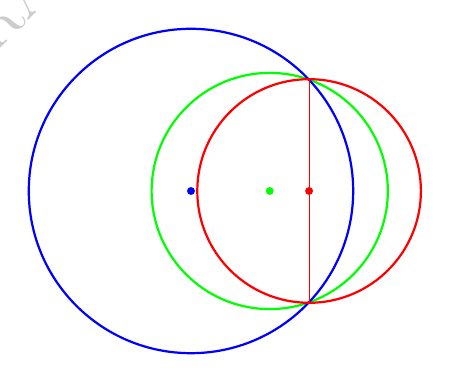
\begin{tikzpicture}[transform shape,scale=1]
	\draw[thick,green] (-1,-1.5) circle (1.5);
	\fill[green] (-1,-1.5) circle (0.5 mm);
	\draw[thick,blue] (-2,-1.5) circle (2.06);
	\fill[blue] (-2,-1.5) circle (0.5 mm);
	\draw[thick,red] (-0.5,-1.5) circle (1.42);
	\fill[red] (-0.5,-1.5) circle (0.5 mm);
	\draw[red](-0.5,-0.0857)--(-0.5,-2.92);	
\end{tikzpicture}\\
\\
\begin{align*}
	S_1\equiv x^2+y^2+2x+3y+1&=0\\
	\\
	S_2\equiv x^2+y^2+4x+3y+2&=0\\
\end{align*}
\\ 
\begin{align*}
S_1-S_2&=0\\
\\
(x^2+y^2+2x+3y+1) - (x^2+y^2+4x+3y+2)& =0\\
\\
x^2+y^2+2x+3y+1-x^2-y^2-4x-3y-2&=0\\
\\
-2x-1&=0\\
\\
2x+1&=0\\
\\
x&=-\frac{1}{2}
\end{align*}
\begin{align*}
x^2+y^2+2x+3y+1&=0\\
\\
\left(-\frac{1}{2}\right)^2+y^2+2\left(-\frac{1}{2}\right)+3y+1&=0\\
\\
\frac{1}{4}+y^2-1+3y+1&=0\\
\\
y^2+3y+\frac{1}{4}&=0\\
\\
y^2+2.\frac{3}{2}.y+\left(\frac{3}{2}\right)^2&=\left(\frac{3}{2}\right)^2-\frac{1}{4}\\
\\
\left(y+\frac{3}{2}\right)^2&=\frac{9}{4}-\frac{1}{4}\\
\\
\left(y+\frac{3}{2}\right)^2&=\frac{8}{4}\\
\\
\left(y+\frac{3}{2}\right)^2&=2\\
\\
y+\frac{3}{2}&=\pm \sqrt{2}\\
\\
y&=-\frac{3}{2}\pm\sqrt{2}\\
\end{align*}
\\ 
নির্ণেয় বৃত্তের ব্যাসের প্রান্ত বিন্দুদ্বয়ের স্থানাঙ্ক $\left(-\frac{1}{2},-\frac{3}{2}+\sqrt{2}\right)$ এবং $\left(-\frac{1}{2},-\frac{3}{2}-\sqrt{2}\right)$\\
\\
\begin{align*}
(x-x_1)(x-x_2)+(y-y_1)(y-y_2)&=0\\
\\
\left(x+\frac{1}{2}\right) \left(x+\frac{1}{2}\right)+\left(y+\frac{3}{2}-\sqrt{2}\right)\left(y+\frac{3}{2}+\sqrt{2}\right)&=0\\
\\
\left(x+\frac{1}{2}\right)^2+\left(y+\frac{3}{2}\right)^2-(\sqrt{2})^2&=0\\
\\
x^2+2.x.\frac{1}{2}+\frac{1}{4}+y^2+2.y.\frac{3}{2}+\left(\frac{3}{2}\right)^2-2&=0\\
\\
x^2+y^2+x+3y+\frac{10}{4}-2&=0\\
\\
x^2+y^2+x+3y+\frac{5}{2}-2&=0\\
\\
x^2+y^2+x+3y+\frac{5-4}{2}&=0\\
\\
x^2+y^2+x+3y+\frac{1}{2}&=0\\
\end{align*}
\\
$\textcolor{green}{x^2+y^2=45}$ বৃত্তের  $(6,-3)$ বিন্দুতে অঙ্কিত স্পর্শক  $\textcolor{blue}{x^2+y^2-4x+2y-35=0}$ বৃত্তকে  A ও  B বিন্দুতে ছেদ করে। দেখাও যে,  A ও B বিন্দুতে স্পর্শকদ্বয় পরস্পর লম্ব। \\
\\  
\begin{tikzpicture}[transform shape,scale=1]
	\draw[thick,green] (0,0) circle (6.7);
	\fill[green] (0,0) circle (0.5 mm);
	\draw[thick,blue] (2,-1) circle (6.32);
	\fill[blue] (2,-1) circle (0.5 mm);
	\fill[red] (6,-3) circle (1 mm);
	\draw[red](4,-7)--(8,1);
	\draw[blue](1,-8)--(10,-5);	
	\draw[blue](7,4)--(10,-5);	
\end{tikzpicture}\\

$x^2+y^2=45$ বৃত্তের  $(6,-3)$ বিন্দুতে অঙ্কিত স্পর্শকের সমীকরণ\\ 
\\ 
\begin{align*}
xx_1+yy_1&=a^2\\
6x+(-3)y&=45\\
6x-3y&=45\\
2x-y&=15\\
y&=2x-15\\
\end{align*}
\begin{align*}
x^2+y^2-4x+2y-35&=0\\
\\
x^2+(2x-15)^2-4x+2(2x-15)-35&=0\\
\\
x^2+4x^2-60x+225-4x+4x-30-35&=0\\
\\
5x^2-60x+160&=0\\
\\
x^2-12x+32&=0\\
\\
x^2-8x-4x+32&=0\\
\\
x(x-8)-4(x-8)&=0\\
\\
(x-8)(x-4)&=0\\
\\
x&=4,8\\
\end{align*}
\begin{align*}
y&=2x-15\\
\\
y&=2(4)-15\\
\\
y&=8-15\\
\\
y&=-7\\
\end{align*}
\begin{align*}
y&=2x-15\\
\\
y&=2(8)-15\\
\\
y&=16-15\\
\\
y&=1\\
\end{align*}
\begin{align*}
x^2+y^2-4x+2y-35&=0\\
\\
x^2+y^2+2(-2)x+2(1)y+(-35)&=0\\
\end{align*}
\begin{align*}
xx_1+yy_1+g(x+x_1)+f(y+y_1)+c&=0\\
\\
x(4)+y(-7)+(-z)(x+4)+(1)(y-7)-35&=0\\
\\
4x-7y-2x-8+y-7-35&=0\\
\\
2x-6y-50&=0\\
\\
x-3y-25&=0\\
\end{align*}
\begin{align*}
xx_1+yy_1+g(x+x_1)+f(y+y_1)+c&=0\\
\\
x(8)+y(1)+(-2)(x+8)+(1)(y+1)-35&=0\\
\\
8x+y-2x-16+y+1-35&=0\\
\\
6x+2y-50&=0\\
\\
3x+y-25&=0\\
\end{align*}
\begin{align*}
xx_1+yy_1+g(x+x_1)+f(y+y_1)+c&=0\\
\\
x(8)+y(1)+(-2)(x+8)+(1)(y+1)-35&=0\\
\\
8x+y-2x-16+y+1-35&=0\\
\\
6x+2y-50&=0\\
\\
3x+y-25&=0\\
\end{align*}
\\
 একটি বৃত্ত $(-1,-1)$ এবং $(3,2)$ বিন্দু দিয়ে অতিক্রম করে এবং এর কেন্দ্র $x^2+y^2-6x-4y-7=0$ বৃত্তের $(1,-2)$ বিন্দুতে স্পর্শকের উপর অবস্থিত । বৃত্তটির সমীকরণ নির্ণয় কর \\ 
 \\ 
 \begin{tikzpicture}[transform shape,scale=1]
 	\draw[thick,green] (3,2) circle (4.47);
 	\fill[green] (3,2) circle (1 mm);
 	\draw[thick,blue] (4,-3.5) circle (5.59);
 	\fill[blue] (4,-3.5) circle (1 mm);
 	\fill[red] (-1,-1) circle (1 mm);
 		\fill[red] (3,2) circle (1 mm);
 	\draw[blue](-3,0)--(7,-5);	
 		\fill[red] (1,-2) circle (1 mm);
 		\node at (-2,-1) {$\textcolor{red}{(-1,-1)}$};	
 		\node at (3,2.5) {$\textcolor{red}{(3,2)}$};
 		\node at (1,-2.5) {$\textcolor{red}{(1,-2)}$};
 		\node at (4,-4) {$\textcolor{blue}{(-g,-f)}$};
 \end{tikzpicture}\\
 \\ 
\begin{align*}
	x^2+y^2-6x-4y-7&=0\\ 
	\\
	x^2+y^2+2(-3)x+2(-2)y+(-7)&=0\\
\end{align*}
\\
\begin{align*}
	xx_1+yy_1+g(x+x_1)+f(y+y_1)+c&=0\\
	\\
	x(1)+y(-2)+(-3)(x+1)-2(y-2)-7&=0\\
	\\
	x-2y-3x-3-2y+4-7&=0\\
	\\
	-2x-4y-6&=0\\
	\\
	x+2y+3&=0\\
	\end{align*}
\\
\begin{align*}
	x^2+y^2+2gx+2fy+c&=0\\
	\\
	(-1)^2+(-1)^2+2g(-1)+2f(-1)+c&=0\\
	\\
	1+1-2g-2f+c&=0\\
	\\
	-2g-2f+c&=-2\\
\end{align*}
\\
\begin{align*}
	x^2+y^2+2gx+2fy+c&=0\\
	\\
	(3)^2+(2)^2+2g(3)+2f(2)+c&=0\\
	\\
	9+4+6g+4f+c&=0\\
	\\
	6g+4f+c&=-13\\
\end{align*}
\\
\begin{align*}
	x+2y+3&=0\\
	\\
	-g+2(-f)+3&=0\\
	\\
	-g-2f+3&=0\\
	\\
	g+2f-3&=0\\
\end{align*}
\\
\begin{align*}
	g=-4,\,\,\,f=\frac{7}{2},\,\,\,c=-3\\
\end{align*}
\\
\begin{align*}
	x^2+y^2+2gx+2fy+c&=0\\
	\\
	x^2+y^2+2(-4)x+2(\frac{7}{2})y-3&=0\\
	\\
	x^2+y^2-8x+7y-3&=0\\
\end{align*}
$x^2+y^2=81$ বৃত্তটির জ্যা  $(-2,3)$ বিন্দুতে সমদ্বিখন্ডিত হয়। জ্যা এর সমীকরণ নির্ণয় কর।\\  
 \begin{tikzpicture}[transform shape,scale=1]
	\draw[thick,green] (0,0) circle (6.36);
	\fill[green] (0,0) circle (1 mm);
	\fill[blue] (-1,1.5) circle (1 mm);
	\draw[blue](-7,-2.5)--(5,5.5);	
		\draw[red](0,0)--(-1,1.5);			
\end{tikzpicture}\\
\begin{align*}
	\frac{x-x_1}{x_1-x_2} &=\frac{y-y_1}{y_1-y_2}\\
	\\
	\frac{x-0}{0+2}&=\frac{y-0}{0-3}\\
	\\
	\frac{x}{2}&=\frac{y}{-3}\\
	\\
	-3x&=2y\\
	\\
	3x+2y&=0\\
\end{align*}
\\
\begin{align*}
	2x-3y+k&=0\\
	\\
	2(-2)-3(3)+k&=0\\
	\\
	-4-9+k&=0\\
	\\
	k&=13\\
\end{align*}
\\
$x^2+y^2=144$ বৃত্তের একটি জ্যা এর সমীকরণ নির্ণয় কর যার মধ্যবিন্দু  $(4,-6)$ বিন্দুতে অবস্থিত। \\ 
\\ 
 \begin{tikzpicture}[transform shape,scale=1]
	\draw[thick,green] (0,0) circle (8.48);
	\fill[green] (0,0) circle (1 mm);
	\fill[blue] (2,-3) circle (1 mm);
	\draw[blue](9.5,2)--(-5.5,-8);	
	\draw[red](0,0)--(2,-3);			
\end{tikzpicture}\\
\begin{align*}
	\frac{x-x_1}{x_1-x_2}&=\frac{y-y_1}{y_1-y_2}\\
	\\
	\frac{x-0}{0-4}&=\frac{y-0}{0+6}\\
	\\
	\frac{x}{-4}&=\frac{y}{6}\\
	\\
	6x&=-4y\\
	\\
	3x+2y&=0\\
\end{align*}
\\
\begin{align*}
	2x-3y+k&=0\\
	\\
	2(4)-3(-6)+k&=0\\
	\\
	8+18+k&=0\\
	\\
	k&=-26\\
\end{align*}
\\
একটি বৃত্তের সমীকরণ নির্ণয় কর যা $y=2$ রেখাকে $(3,2)$ বিন্দুতে স্পর্শ করে এবং $(1,4)$ বিন্দু দিয়ে যায়। \\
\\
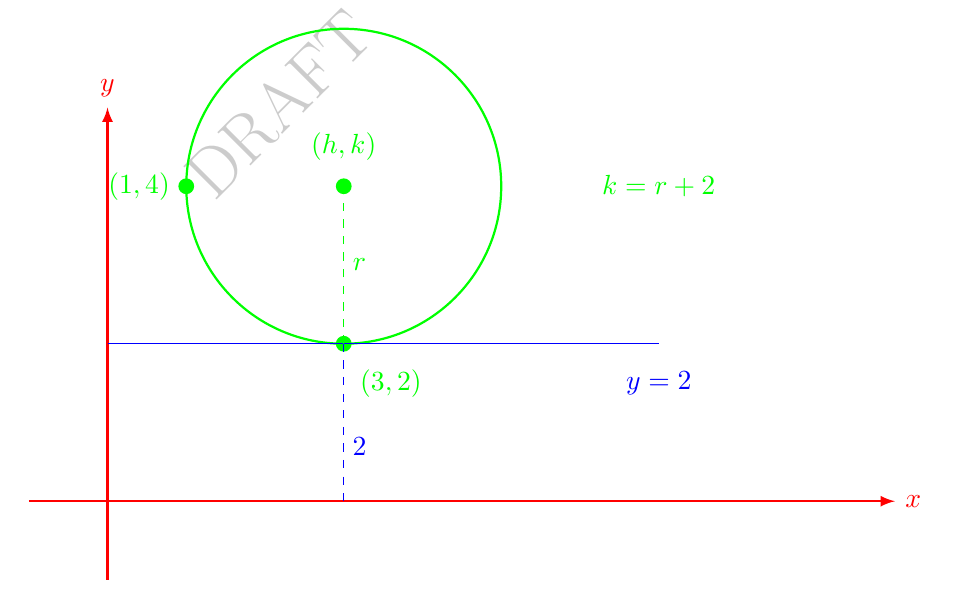
\begin{tikzpicture}[transform shape,scale=1]
	\draw [-latex,thick,red](-1,0) -- (10,0) node[right] {$x$} coordinate(x axis);
	\draw [-latex,thick,red](0,-1) -- (0,5) node[above] {$y$} coordinate(y axis);
	\draw[thick,green] (3,4) circle (2);
	\fill[green] (3,4) circle (1 mm);
	\fill[green] (3,2) circle (1 mm);
	\fill[green] (1,4) circle (1 mm);
	\draw[blue](0,2)--(7,2);
	\draw[blue,dashed](3,2)--(3,0);
	\draw[green,dashed](3,2)--(3,4);	
	\node at (3.6,1.5) {$\textcolor{green}{(3,2)}$};
	\node at (0.4,4) {$\textcolor{green}{(1,4)}$};	
	\node at (7,1.5) {$\textcolor{blue}{y=2}$};
	\node at (3,4.5) {$\textcolor{green}{(h,k)}$};
	\node at (3.2,0.7) {$\textcolor{blue}{2}$};
	\node at (3.2,3) {$\textcolor{green}{r}$};
	\node at (7,4) {$\textcolor{green}{k=r+2}$};
\end{tikzpicture}\\
\\ 
\begin{align*}
	(x-h)^2+(y-k)^2&=r^2\\
	\\
	(x-3)^2+(y-k)^2&=(k-2)^2\\
	\\
	(1-3)^2+(4-k)^2&=(k-2)^2\\
	\\
	(-2)^2+16-8k+k^2&=k^2-4k+4\\
	\\
	4k&=16\\
	\\
	k&=4
\end{align*}
\end{document}